\documentclass[10pt,letterpaper]{article}
\usepackage{fullpage}
%\usepackage[top=2cm, bottom=4.5cm, left=2.5cm, right=2.5cm]{geometry}
\usepackage[letterpaper, portrait, left=1in, right=1in, top=1in, bottom=1.5in]{geometry}
\usepackage{amsmath,amsthm,amsfonts,amssymb,amscd, bm}
\usepackage{mlmodern}
\usepackage{amsmath}
\usepackage{amssymb}
\usepackage{amsthm}
\usepackage{lastpage}
\usepackage{enumerate}
\usepackage{fancyhdr}
\usepackage{mathrsfs}
\usepackage{xcolor}
\usepackage{graphicx}
\usepackage{listings}
\usepackage{hyperref}
\usepackage{wrapfig}
\usepackage{siunitx}
\usepackage{enumitem}
\usepackage{multicol}
\usepackage{float}
\hypersetup{%
  colorlinks=true,
  allcolors=blue
}

\title{Statistical Visualization of Strength Measurement Formulas Across Powerlifting}
\author{Ricardo A. Miranda}


\begin{document}
    \maketitle
    \begin{center}
        \textbf{Project Summary}
    
    \end{center}
    The purpose of this project is to show the differences in strength systems that are used to measure strength of lifters across different genders and weight classes. To this day, there are ongoing conversations of how to measure strength of a lifter in order to dictate what feats are considered ``best". This project serves to provide a brief overview of the current systems in place and choose the best system overall based on the data points worked with.

    \tableofcontents

    \newpage

    \section{Summary of Powerlifting}
    Powerlifting is an up and coming popular sport that has been gaining traction in the last few decades. It is considered a strength sport that involves a barbell, similar to olympic weightlifting, expect it focuses on the 3 compound lifts: squat, bench press, and deadlift. In a typical competition, powerlifters come together in a meet and have a total of 9 attempts, 3 for each lift, in order to acheive the maximum total possible. A 4th lift is permitted if the 4th lift is an attempt at breaking a current record but it does not count towards the lifter's total. The lifters are placed into their respective weight classes based on how much they weighed prior to the competition during their weigh-in period. These weight classes differ depending on the federation that they compete in. The federation that we are focusing on in this paper is USA Powerlifting (USAPL). The type of powerlifting we are focusing on is classic or raw, which refers to the type of equipment that is allowed to be used in competition and the number of lifts that are expected to be done at the meet. For the particular meet we are looking at, all three lifts were expected to be performed. The equipment that was allowed for this meet were permitted singlets, lifting belts, and wrist wraps.
    \subsection*{Squat}
    The squat is the first lift in a typical powerlifting meet. It requires a lifter to place a bar on their back and squatting to the point where the top of their knee is in line with their hip crease (the hip crease can be lower but it must reach the top of the knee at minimum) in order to be considered a ``good'' lift. This is a standard that is required for all lifters to do, otherwise the lift is disqualified from counting towards their total.
    \subsection*{Bench Press}
    The bench press is the second lift in a typical powerlifting meet. It requires a lifter to be in a face-up prone position on a bench. The lifter takes a bar in their hands and allows the bar to descend until the bar touches a point on their torso (wherever that may be). The lifter must hold the bar in that position until given a command to press by a ref. If the command is not followed, the lift is disqualified from counting towards their total. 
    \subsection*{Deadlift}
    The deadlift is the third and last lift in a typical powerlifting meet. The standards for this lift aren't as rigourous as the others. A lifter simply has to reach down and lift a bar until they are completely upright. If the bar shows any downward movement during the lift, it is disqualified from counting towards their total.
    \subsection*{Rankings}
    At the end of a meet, the lifter with the highest total in their weight class wins for their respective weight class. However, the lifter with the highest score based on a strength formula can be given to whichever lifter has the highest relative score. The current metric that USAPL uses is IPF GL formula or the GL formula. Prior to 2019, USAPL used the Wilks Formula to generate a Wilks score.

    \newpage 
    \section{The Different Strength Metrics}
    There are various strength metrics that have been used to judge relative strength scores across weight classes. They have primarily been used to give awards for ``best'' lifter all around at a particular meet. The need for strength scores are not necessary unless one wishes to compare lifters' performances across different weight classes. 
    
    Using absolute total, i.e. whoever lifts the highest total, regardless of weight class, is the best lifter, or using a bodyweight multiplier score, i.e. whoever has the highest ratio of total to bodyweight is the best lifter, can easily be shown to be skewed to heavier lifters and lighter lifters, respectively. 
    
    The goal of powerlifting federations has been to provide a fair metric where there are no advantages whether you are a lightweight or superheavy weight, male or female, etc. This is discussed on the IPF page \cite{ipfPage}.

    We will be looking at 7 different graphs, one for each metric. The x-axis will be the weight of the lifter in kilograms and the y-axis will be the proposed method of measuring strength. The variables for the y-axis are: total, body weight multiplier, wilks score, wilks-2 score, DOTS score, IPF, and GL. All of these formulas/variables have been used as a measure of strength in competition before and/or is used in the fitness industry as measures of strength. Currently, absolute total is used within the same weight class but GL is used to generate a score for everyone across all weight classes. For any graphs, we do not want to see any type of linear relationship. All formulas used can be found \href{https://www.powerlifting.sport/fileadmin/ipf/data/ipf-formula/Models_Evaluation-I-2020.pdf}{here}.

    The data used for the creation of these graphs was obtained at \cite{data}. This is a database where USAPL stores all data regarding powerlifitng meets. The meet we are looking at is Raw Nationals which took place on June 14, 2021. This meet provided 84 data points for men and 74 data points for women for a total of 158 data points.

    \subsection{Strength Metric: Absolute Total}
    The first metric we will look at is simply the total that a lifter achieves. As mentioned before, using this metric becomes noticeably skewed towards the heavier lifters at a meet. A graph of bodyweight versus total is shown below. 

    \begin{figure}[H]
        \center 
        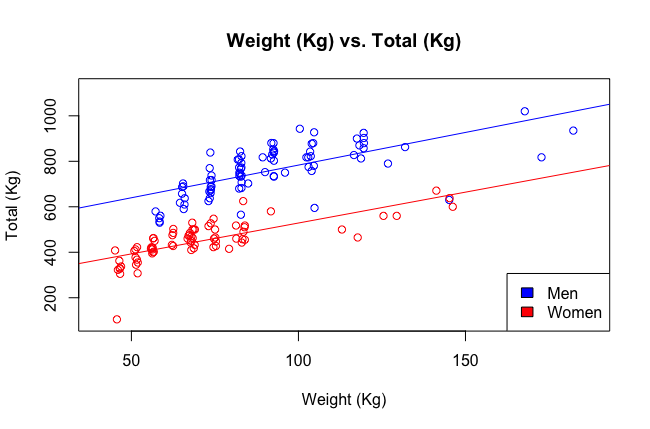
\includegraphics[width=35em]{weightVStotal.png}
        \label{total}
    \end{figure}

    It is noticeable that there is an increasing linear relationship between weight and total. The higher the weight, the higher the total, typically. You can also see that men almost always have higher totals than women.
    Using a few tools from R, we find that the correlation between the two variables is 0.667 for men and 0.743 for women. We can also create a linear regression formula for a prediction of ``Total" using the weight of the lifter based on the data provided:
    \begin{align*}
    Total_{m} &= 2.87BW + 495.96, \\
    Total_{w} &= 2.71BW + 257.08
    \end{align*}

     A trendline has also been graphed based on this formula. With this information, we can conclude that it would not be fair towards lighter lifters and women to use absolute total as a strength metric. 

    \subsection{Strength Metric: Bodyweight Multiplier}
    The second metric we will look at is a bodyweight multipler of amount of weight lifter compared to body weight. The formula for calculating the bodyweight multiplier is: $$xBW = \frac{Total}{BW}$$ where $Total$ and $BW$ are measured in kilograms. A graphic of bodyweight versus bodyweight multiplier is shown below. 

    \begin{figure}[H]
        \center
        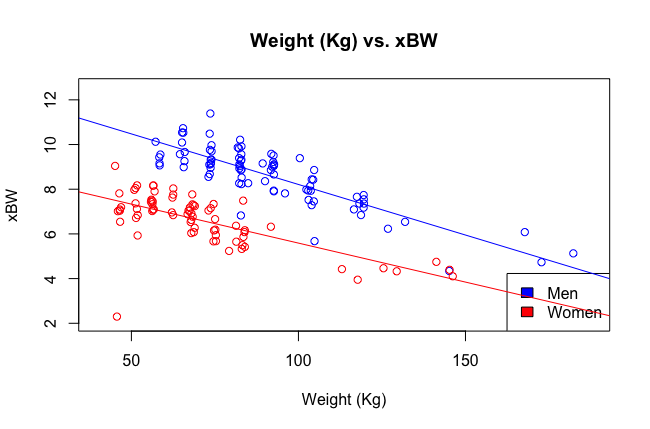
\includegraphics[width=35em]{weightVSbw.png}
        \label{xBW}
    \end{figure}

    It is noticeable that there is a decreasing linear relationship between weight and bodyweight multiplier. The lower the weight, the higher the bodyweight multiplier score, typically. You can also see that men almost always have a higher bodyweight multiplier than women. We find that the correlation between the two variables are -0.838 for men and -0.681 for women. The linear regression formulas for both men and women are: 
    \begin{align*}
        xBW_{m} &= -0.045BW + 12.74, \\
        xBW_{w} &= -0.035BW + 9.079
        \end{align*}
    
    A trendline has also been graphed based on this formula. We can conclude that it would not be fair towards heaiver lifters and women to use a bodyweight multiplier score as a strength metric.
    
    \subsection{Strength Metric: Wilks Formula}
    The third metric we will look at is the Wilks Formula or the Wilks Coefficients. The formula for calculating the wilks score is 
    \begin{align*}
        Wilks \ Score = Total \cdot \frac{500}{A \cdot BW^5 + B \cdot BW^4 + C \cdot BW^3 + D \cdot BW^2 + E \cdot BW + F}
    \end{align*}
    where coefficients for men are:
    \begin{flalign*}
        &A = -0.00000001291& \\
        &B = 0.00000701863& \\
        &C = -0.00113732& \\
        &D = -0.002388645& \\
        &E =  16.2606339& \\
        &F = -216.0475144&
    \end{flalign*}
    and coefficients for women are: 
    \begin{flalign*}
        &A = -0.0000009054& \\
        &B = 0.00004731582& \\
        &C = -0.00930733913& \\
        &D = 0.82112226871& \\
        &E =  27.23842536447& \\
        &F = 594.31747775582&
    \end{flalign*}
    A graph of bodyweight versus wilks score is found below. 

    \begin{figure}[H]
        \center
        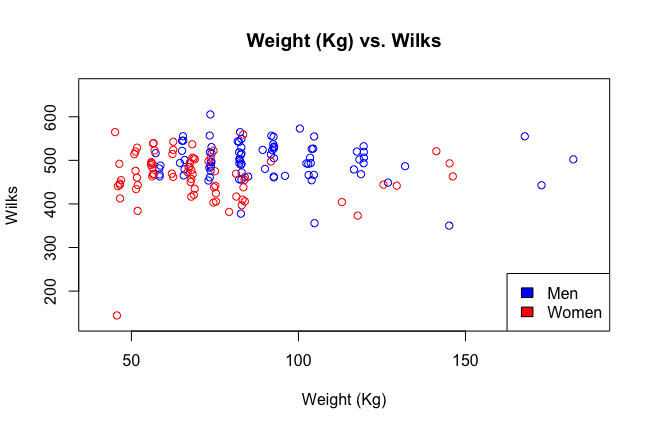
\includegraphics[width=35em]{weightVSwilks.png}
        \label{wilks}
    \end{figure}

    You can see in this figure that any linear relationship that we have seen before has reduced greatly. You can also see that scores amongst men and women are now more similar to one another than they were before. The correlation between weight and wilks for men is -0.144 and for women is -0.059.

    \subsection{Strength Metric: Wilks-2 Formula}
    The fourth metric we will look at is the Wilks-2 formula. This is an update to the previous Wilks formula. I suspect that this update occurred because more and more elite level athletes kept brekaing records and thus the coefficients needed to take into account the new data points. The formula for calculting the wilks-2 score is:
    \begin{align*}
        Wilks-2 \ Score = Total \cdot \frac{600}{A \cdot BW^5 + B \cdot BW^4 + C \cdot BW^3 + D \cdot BW^2 + E \cdot BW + F}
    \end{align*}
    where coefficients for men are:
    \begin{flalign*}
        &A = -0.0000000120804336482315& \\
        &B = 0.00000707665973070743& \\
        &C = -0.00139583381094385& \\
        &D = 0.073694103462609& \\
        &E = 8.47206137941125& \\
        &F = 47.4617885411949&
    \end{flalign*}
    and coefficients for women are: 
    \begin{flalign*}
        &A = -0.000000023334613884954& \\
        &B = 0.00000938773881462799& \\
        &C = -0.0010504000506583& \\
        &D = -0.0330725063103405& \\
        &E = 13.7121941940668& \\
        &F = -125.425539779509&
    \end{flalign*}
    A graph of bodyweight versus wilks-2 score is found below. 

    \begin{figure}[H]
        \center
        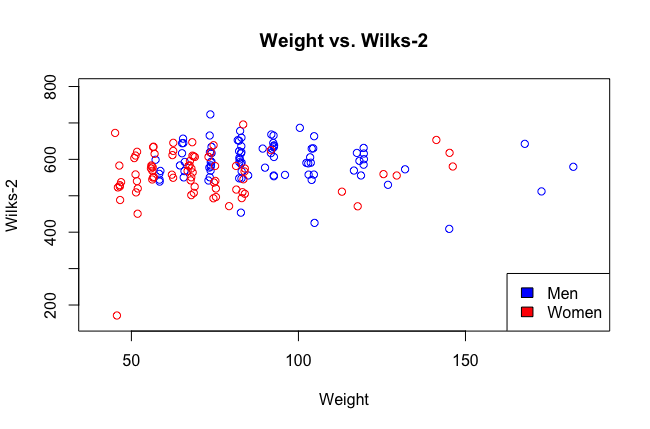
\includegraphics[width=35em]{weightVSwilks2.png}
        \label{wilks2}
    \end{figure}
    This graph looks somewhat similar to \ref{wilks} however women tend to have a higher score with the wilks-2 formula, perhaps making it a more fair metric for women compared to the original wilks formula. The correlation between weight and Wilks-2 is -0.172 for men and 0.106 for women. 

    \subsection{Strenght Metric: DOTS Formula}
    The fifth metric we will look at is the DOTS formula. It looks similar to the wilks formula. The formula for calculating the DOTS score is: 
    \begin{align*}
        DOTS \ Score = Total \cdot \frac{500}{A \cdot BW^4 + B \cdot BW^3 + C \cdot BW^2 + D \cdot BW + E}
    \end{align*}
    where coefficients for men are:
    \begin{flalign*}
        &A = -0.000001093& \\
        &B = 0.0007391293& \\
        &C = -0.1918759221& \\
        &D = 24.0900756& \\
        &E = -307.75076&
    \end{flalign*}
    and coefficients for women are: 
    \begin{flalign*}
        &A = -0.0000010706& \\
        &B = 0.0005158568& \\
        &C = -0.1126655495& \\
        &D = 13.6175032& \\
        &E = -57.96288&
    \end{flalign*}
    A graph of bodyweight versus DOTS score is found below. 

    \begin{figure}[H]
        \center
        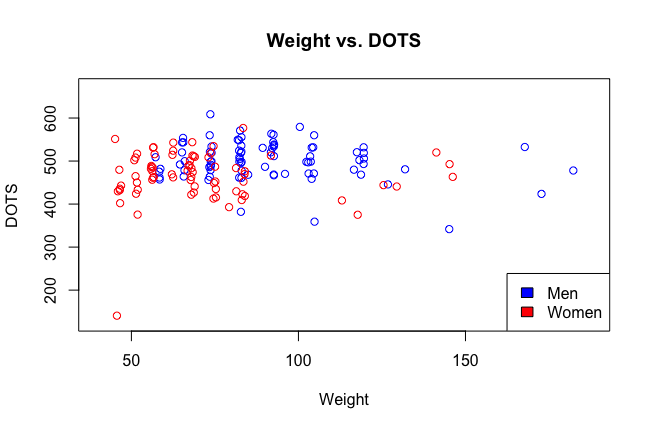
\includegraphics[width=35em]{weightVSdots.png}
        \label{dots}
    \end{figure}
    This graph and the original wilks graph \ref{wilks} look nearly identical. The correlation between the weight and DOTS is -0.202 for men and 0.0131 for women.  

    \subsection{Strength Metric: IPF Formula}
    The sixth metric we will look at is the IPF Formula. This is the current metric that is used in USAPL meets as well as IPF competitions. The formula for this metric also looks greatly different compared to the ones we have seen before. The formula for calculating an IPF score is: 
    \begin{align*}
        IPF \ Score = 500 + 100 \cdot \frac{Total - (A \cdot \ln(BW) - B)}{C \cdot \ln(BW) - D}
    \end{align*}
    The coefficients for men and women are based on the type of competition that is being done. In this case, we will use the coefficients for classic powerlifting or raw powerlifting. The coefficients for men are: 
    \begin{flalign*}
        &A = 310.6700& \\
        &B = 857.7850& \\
        &C = 53.2160& \\
        &D = 147.0835&
    \end{flalign*}
    and the coefficients for women are: 
    \begin{flalign*}
        &A = 125.1435& \\
        &B = 228.0300& \\
        &C = 34.5246& \\
        &D = 86.8301&
    \end{flalign*}
    A graph of bodyweight versus IPF score is found below: 
    \begin{figure}[H]
        \center
        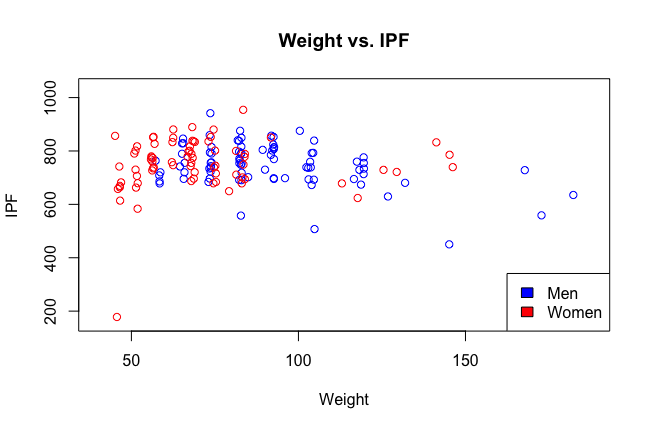
\includegraphics[width=35em]{weightVSipf.png}
        \label{ipf}
    \end{figure}
    This graph shows a noticeable increase of scores for women compared to men. In all previous graphs, the highest score belong to a man. In this graph, that score now belongs to a woman. The correlation between weight and IPF is -0.392 for men and 0.104 for women. 

    \subsection{Strength Metric: GL Formula}
    The seventh and last metric we will look at is the GL Formula. This formula also looks different than the rest and is the first to introduce an exponential. The formula is:
    \begin{align*}
        GL \ Score = Total \cdot \frac{100}{A - B \cdot e^{-C \cdot BW}}
    \end{align*}
    The coefficients for classic powerlifting for men are: 
    \begin{flalign*}
        &A = 1199.72839& \\
        &B = 1025.18162& \\
        &C = 0.00921&
    \end{flalign*}
    and the coefficients for women are: 
    \begin{flalign*}
        &A = 610.32796& \\
        &B = 1045.59282& \\
        &C = 0.03048&
    \end{flalign*}
    A graph of bodyweight versus GL score is found below: 
    \begin{figure}[H]
        \center
        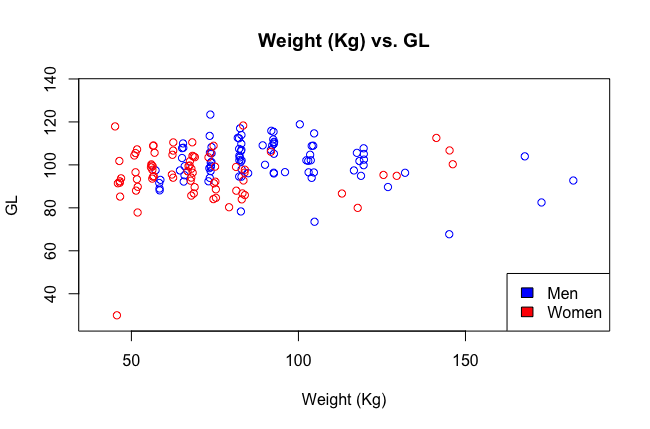
\includegraphics[width=35em]{weightVSgl.png}
        \label{gl}
    \end{figure}
    This graph shows simlar results to the Wilks-2 graph \ref{wilks2}. The correlation between weight and GL points is -0.184 for men and 0.078 for women.


    \section{Discussion of Results}
    In the previous section, we looked at the different strength metrics that one could use. We quickly saw that the first two, absolute total \ref{total} and body weight multiplier \ref{xBW}, showed a high correlation between weight and the variable in question. Both favored men over women as the stronger relative lifter.

    All the other metrics seemed to serve as much better metric in comparison to the first two as correlation between weight and the metric used went down significantly. However, if you look closely, all graphs except the IPF graph \ref{ipf} show clusters of women scoring noticeably below men in their respective weight classes. Whether this means that men are typically stronger relative lifters in comparison than women, I am not sure of but this could show a potential bias towards men in these formulas. 
    
    The metric that had the lowest correlation for men and women in separate groups was the original Wilks formula. 


    In terms of which metric is ``best'', the paper where the formulas were found conduct an evaulation of these strength metrics. The authors Kopayev, Onyschenko, and Stetsenko come to the conclusion that the GL formula is the best metric to use \cite{formulas}. 


    \newpage
    \section{RStudio Code, Data, and GitHub}
    The R code used to generate the results in the graphs are below. I used a series of for loops in order to generate the graphs quickly as opposed to plotting them one by one. You can find this code on my \href{https://github.com/mirandaricky9/math353DataVisualization}{GitHub} as well as the R Project.

    \begin{verbatim}
n = names(Mens)
metrics <- n[4:10]
x_0 = Mens[[n[2]]] # this is the x axis, it will always be weight
x_1 = Womens[[n[2]]]
for (i in 4:10) {
    y_0 = Mens[[n[i]]] # this is the y axis, will go from total to GL
    y_1 = Womens[[n[i]]]
    label = n[i]
    if (label == 'Total'){
    label = paste(label, '(Kg)', sep = ' ')
    }
    plot(x_0, y_0, xlab = 'Weight (Kg)', ylab = label, main = paste(n[2],
    label, sep=" (Kg) vs. ") , xlim = c(min(Womens$Weight) - 5, 
    max(Mens$Weight) + 5), ylim = c(min(y_1) - min(y_1)*0.1, 
    max(y_0) + max(y_0)*0.1), col = 'blue')
    points(x_1, y_1, col = 'red')
    legend(x = "bottomright", legend=c("Men", "Women"), 
            fill = c("blue","red"))
    if (label == 'Total (Kg)'){ # adding trend lines
    abline(lm(formula = Total ~ Weight, data = Mens), col = 'blue')
    abline(lm(formula = Total ~ Weight, data = Womens), col = 'red')
    }
    else if (label == 'xBW') {
    abline(lm(formula = xBW ~ Weight, data = Mens), col = 'blue')
    abline(lm(formula = xBW ~ Weight, data = Womens), col = 'red')
    }

}
. . .
    \end{verbatim}
The rest of the code can be found in the GitHub repository if interested.

The data that was used for this project was stored on an excel file. The file contained columns for the lifters name, weight, weight class, their total, as well as scores for all metrics seen above. The data on the excel file was imported into R to look at. Both the excel file and the RProject can be found on the GitHub Repository. 

    %Add some info regarding the tools used. 
    % Another observation that can be made is that the metric might be skewed towards women in the lighter weight classes 
    % and skewed towards males in the middle and heavier weight classes.
    % Talk about the means that for each one
    % Talk about worklog in the executive summary 
    % include a trend line for the graphs that show linearity 

    \section*{Executive Summary}


    \newpage
    \begin{thebibliography}{}
        \bibitem{formulas}
        Oleksandr Kopayev, Borys Onyschenko, Anatoliy Stetsenko,
        \textit{Evaluation of Wilks, Wilks-2, DOTS, IPF and Goodlift formulas for calculating relative scores in IPF powerlifting
        competitions}, Powerlift.Sport, https://www.powerlifting.sport/fileadmin/ipf/data/ipf-formula/Models-Evaluation-I-2020.pdf, Accesssed April 2022
        
        \bibitem{data}
        No Author Available,
        \textit{USAPL}, USAPL Lifting Databases, https://usapl.liftingdatabase.com/competitions-view?id=119704, Accessed April 2022
        

        \bibitem{ipfPage}
        No Author Available,
        \textit{IPF}, Powerlifting Sport, https://www.powerlifting.sport/rules/codes/info/ipf-formula, Accessed April 2022
    \end{thebibliography}
\end{document}